%%%%%%%宏包定义区%%%%%%%%%%%%%%%%%%%%%%%%%%%%%%%%%%%%%%%%%%%%%%%%%%%%%%%%%%%%%%%%%%%
\documentclass[12pt,a4paper,twoside]{article}
\usepackage[UTF8]{ctex}
\usepackage[T1]{fontenc}
\usepackage{amsmath, esint}
\usepackage{amsfonts}
\usepackage{listings}
\usepackage{amssymb}
\usepackage{soul, color}
\usepackage{cancel}
\usepackage{wrapfig}
\usepackage[left=2.54cm, right=2.54cm, top=2.54cm, bottom=2.54cm]{geometry}
\usepackage[colorlinks,linkcolor=cyan]{hyperref}
\linespread{1.0}
\usepackage{graphicx}

%%%%%%%%%%%%%%%%%%%%%%%%%%%%%%%%%%%%%%%%%%%%%%%%%%%%%%%%%%%%%%%%%%%%%%%%%%%%%%%%%%%%%%%%%%%%%%
% Define the header.
\usepackage{fancyhdr}
\pagestyle{fancy}
\fancyhf{}
\fancyhead[RE,RO]{\leftmark} % Define header: LE= Left in Even pages, RE = Right in Even pages. CO = Center in Odd pages. \leftmark = section number and section name
\fancyhead[LE,LO]{\LaTeX\ \textsc{Template for Notes}}
\fancyfoot[CE,CO]{\thepage}
%%%%%%%%%%%%%%%%%%%%%%%%%%%%%%%%%%%%%%%%%%%%%%%%%%%%%%%%%%%%%%%%%%%%%%%%%%%%%%%%%%%%%%%%%%%%%%
% Define Griffith's script r (PHY250/350)
\usepackage{tikz}
\usetikzlibrary{arrows,scopes}
\newcommand{\rc}{
\resizebox{!}{1.25ex}{
    \begin{tikzpicture}[>=round cap]
        \clip (0.09em,-0.05ex) rectangle (0.61em,0.81ex);
        \draw [line width=.11ex, <->, rounded corners=0.13ex] (0.1em,0.1ex) .. controls (0.24em,0.4ex) .. (0.35em,0.8ex) .. controls (0.29em,0.725ex) .. (0.25em,0.6ex) .. controls (0.7em,0.8ex) and (0.08em,-0.4ex) .. (0.55em,0.25ex);
    \end{tikzpicture}
}
}

\newcommand{\brc}{
\resizebox{!}{1.3ex}{
    
\begin{tikzpicture}[>=round cap]
        \clip (0.085em,-0.1ex) rectangle (0.61em,0.875ex);
        \draw [line width=.2ex, <->, rounded corners=0.13ex] (0.1em,0.1ex) .. controls (0.24em,0.4ex) .. (0.35em,0.8ex) .. controls (0.29em,0.725ex) .. (0.25em,0.6ex) .. controls (0.7em,0.8ex) and (0.08em,-0.4ex) .. (0.55em,0.25ex);
    \end{tikzpicture}
}
}
\newcommand{\hrc}{\hat{\brc}}
%%%%%%%%%%%%%%%%%%%%%%%%%%%%%%%%%%%%%%%%%%%%%%%%%%%%%%%%%%%%%%%%%%%%%%%%%%%%%%%%%%%%%%%%%%%%%%
% Make the equation numbering become "(section number.equation #)"
\numberwithin{equation}{section}
%%%%%%%%%%%%%%%%%%%%%%%%%%%%%%%%%%%%%%%%%%%%%%%%%%%%%%%%%%%%%%%%%%%%%%%%%%%%%%%%%%%%%%%%%%%%%%
% Code listing from Overleaf.
\definecolor{codegreen}{rgb}{0,0.6,0}
\definecolor{codegray}{rgb}{0.5,0.5,0.5}
\definecolor{codepurple}{rgb}{0.58,0,0.82}
\definecolor{backcolour}{rgb}{0.95,0.95,0.92}

\lstdefinestyle{mystyle}{
    backgroundcolor=\color{backcolour},   
    commentstyle=\color{codegreen},
    keywordstyle=\color{magenta},
    numberstyle=\tiny\color{codegray},
    stringstyle=\color{codepurple},
    basicstyle=\ttfamily\footnotesize,
    breakatwhitespace=false,         
    breaklines=true,                 
    captionpos=b,                    
    keepspaces=true,                 
    numbers=left,                    
    numbersep=5pt,                  
    showspaces=false,                
    showstringspaces=false,
    showtabs=false,                  
    tabsize=2
}
\lstset{style=mystyle}
%%%%%%%%%%%%%%%%%%%%%%%%%%%%%%%%%%%%%%%%%%%%%%%%%%%%%%%%%%%%%%%%%%%%%%%%%%%%%%%%%%%%%%%%%%%%%%

%%%%%%%%%%%%%%%%%%%%%%%%%正文分界线,上面全是模板%%%%%%%%%%%%%%%%%%%%%%%%%%%%%%%%%%%%%%%
\everymath{displaystyle}
\begin{document}  %%文件开始%%

%标题%
\begin{center}
		\textbf{\Large{\LaTeX \ Template for Math and Physics notes}}\\
		\textit{Kuzma Cosmos (2022)}
	\end{center}
 
%\section{}表示分部分%
\section{设置 \LaTeX}

\begin{itemize}
    \item 个人使用Overleaf在线编辑实验报告,优点是不用手动添加各种宏包,很多package Overleaf都是有的。缺点是离线无法保存。网址:\href{https://www.overleaf.com/project}{传送门};

    \item 在Overleaf网站创建一个账号,或者使用google等账号授权登录,这样就进入了Overleaf的主页面。

    \item 点击左上角绿色的“New Project”,就进入了新文档页面。一般选择空白project(Blank project),然后复制粘贴模板。

    \item 点击左上角带有Overleaf 标志+Menu的选项,进入文件配置设置。如果全英文,则去掉这个pdf文档的tex代码文件的第三排:
    \begin{verbatim}\usepackage[UTF8]{ctex} \end{verbatim}
    
    如果想写中英文混合,选择"XeLaTeX",并保留这个pdf文档的tex代码文件的第三排代码。

    \item 然后就可以自由编辑啦!

    \item \LaTeX 数学公式生成器:\href{https://latex.codecogs.com/eqneditor/editor.php}{传送门。}
    
\end{itemize}


\newpage %强制换页

\section{各种例子——数学}

\subsection{Jacobian}
This is the equation for changing variable in double integral:

\begin{equation}
    \iint_{\mathcal{S}}f(x,y) dxdy = \iint_{\mathcal{D}}f(x(u, v),\ g(u,v))\left|\dfrac{\partial(x,y)}{\partial(u,v)}\right|dudv
    \label{eq: change-variable-double-int} % 公式的标签,引用公式时需要使用这个标签。
\end{equation}

where $(x,y)=T(u,v)=(x(u,v),\ y(u,v))$ with a defined transformation $T: \mathcal{D}\to \mathcal{S}$. $\dfrac{\partial(x,y)}{\partial(u,v)}$ is called (determinant of) \textbf{Jacobian} of $T$, denoted by $\mathrm{Jac}(T)$:

\begin{equation} %%公式开始
    \boxed{ %% 这个公式加了方框
    |\mathrm{Jac}(T)| = \frac{\partial(x,y)}{\partial(u,v)} =
    \def\arraystretch{2}
    \begin{vmatrix}
    \dfrac{\partial x}{\partial u} & \dfrac{\partial x}{\partial v}\\ 
    \dfrac{\partial y}{\partial u} & \dfrac{\partial y}{\partial v}
    \end{vmatrix}
    }
\end{equation} %%公式结束

\noindent The equation of Jacobian matrix determinant is Eq. \ref{eq: change-variable-double-int}.\\ % \noindent 表示不缩进(四格), \ref{} 表示referring to xxx(figure, equation, etc) with a label. "\\"表示强制断行进入下一行

\noindent Below is an example of inserting picture.
\begin{figure}[ht] % ht = here or top
    \centering %居中
    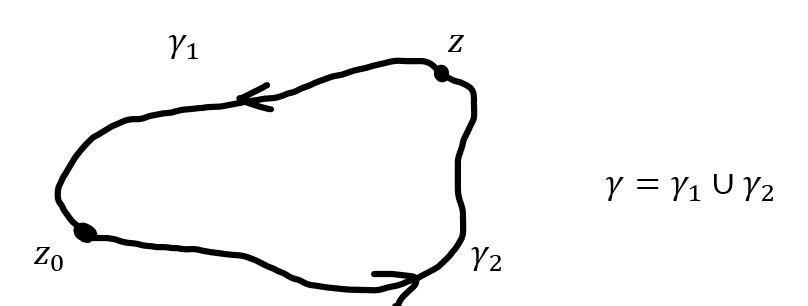
\includegraphics[width = 10cm]{closed-curve-two-points.png} % width/height 参数可以自定义
    \caption{Sample picture} %图片名称
    \label{fig: sample} %图片标签
\end{figure}

\noindent 注意上图的名称是“图一:Sample picture”,因为我们之前设置了中文语言环境。如果需要全英文,则需要删除这行命令:\begin{verbatim}\usepackage[UTF8]{ctex} \end{verbatim}
\newpage %强制新建页

\section{物理例子}
\subsection{Biot-Savart Law}
This is equation for Biot-Savart Law in magnetostatics, from Griffiths' Textbook.
\begin{equation}
    \boxed{
    \overrightarrow{B} = \dfrac{\mu_0}{4\pi}\int_{\mathcal{W}}\dfrac{\overrightarrow{I}\times \hrc}{\rc^2}dl=\dfrac{\mu_0I}{4\pi}\int_{\mathcal{W}}\dfrac{d\overrightarrow{l}\times \hrc}{\rc^2}
    }
    \label{Eq: Biot-Savart}
\end{equation}


\newpage %强制新建页

\section{Python codes in \LaTeX}
Sample python code.
\lstinputlisting[language = Python]{sample.py} %导入整个python代码的line of code

\end{document}